\chapter{Basics}

\section{Design and Philosophy}

The main idea of the PARALUTION objects is that they are separated from the actual hardware specification. Once you declare a matrix, a vector or a solver, they are initially allocated on the host (CPU). Then, every object can be moved to a selected accelerator by a simple move-to-accelerator function. The whole execution mechanism is based on run-time type information (RTTI) which allows you to select where and how you want to perform the operations at run time. This is in contrast to the template-based libraries which need this information at compile time. 

The philosophy of the library is to abstract the hardware-specific functions and routines from the actual program which describes the algorithm. It is hard and almost impossible for most of the large simulation software based on sparse computation to adapt and port their implementation in order to use every new technology. On the other hand, the new high performance accelerators and devices have the capability to decrease the computational time significantly in many critical parts. 

This abstraction layer of the hardware specific routines is the core of PARALUTION's design, it is built to explore fine-grained level of parallelism, suited for multi/many-core devices. This is in contrast to most of the parallel sparse libraries available which are mainly based on domain decomposition techniques. Thus, the design of the iterative solvers and preconditioners is very different. Another cornerstone of PARALUTION is the native support of accelerators - the memory allocation, transfers and specific hardware functions are handled internally in the library.

PARALUTION helps you to use accelerator technologies but does not force you to use them. As you can see later in this chapter, even if you offload your algorithms and solvers to the accelerator device, the same source code can be compiled and executed in a system without any accelerators.

\section{Operators and Vectors}

The main objects in PARALUTION are linear operators and vectors. All objects can be moved to an accelerator at run time -- a structure diagram is presented in Figure~\ref{class-backends}. Currently, PARALUTION support GPUs by CUDA (NVIDIA) and OpenCL (NVIDIA, AMD) backends and provides an OpenMP MIC backend for the Intel Xeon Phi.


\begin{figure}[!ht]
\centering
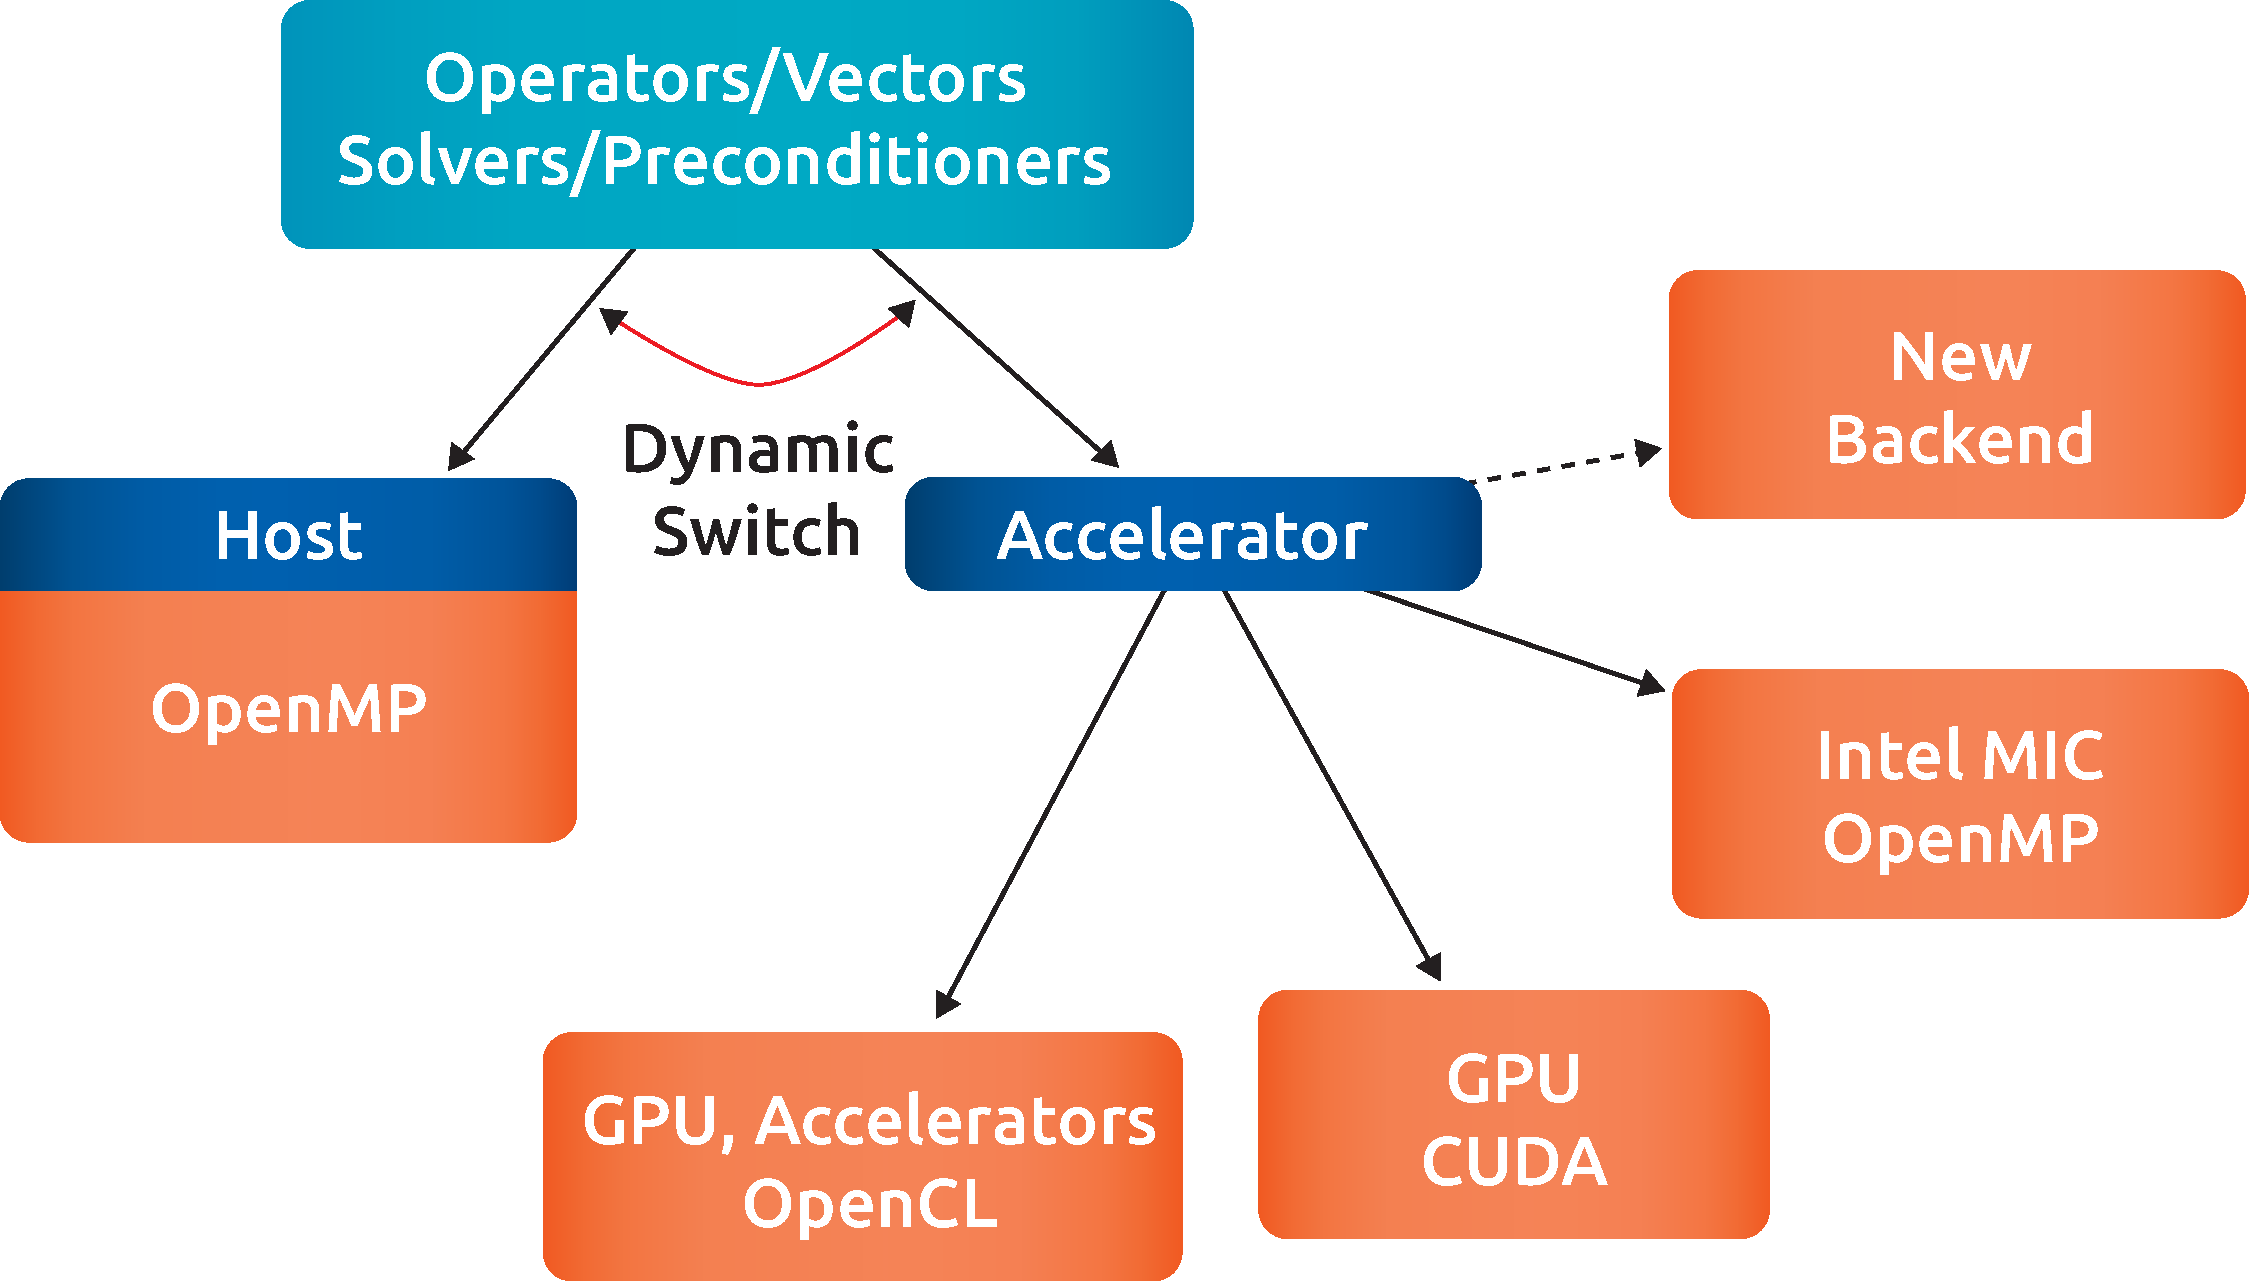
\includegraphics[width=0.6\textwidth]{./fig/structure.pdf}
\caption{Host and backends structure for different hardware}
\label{class-backends}
\end{figure}


The linear operators are defined as local or global matrices (i.e. on a single node or distributed/multi-node) and local stencils (i.e. matrix-free linear operations). 

\begin{figure}[!ht]
\centering
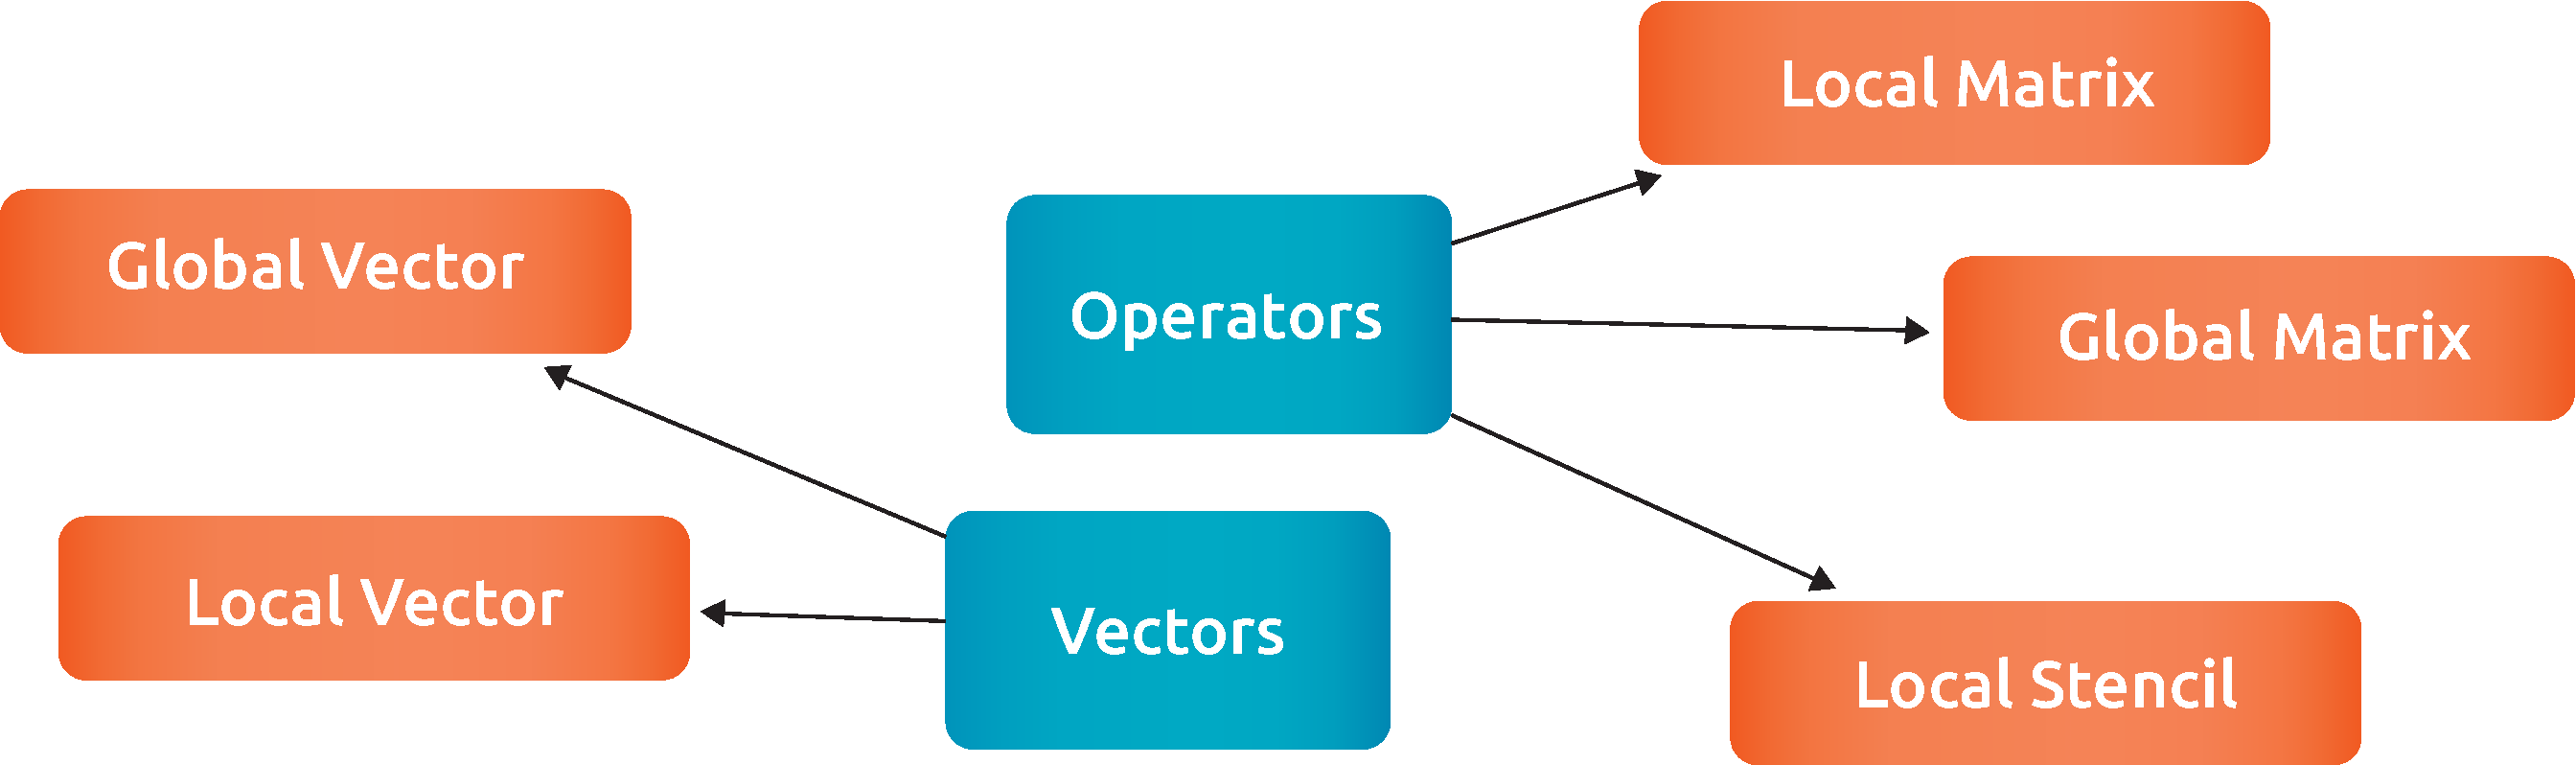
\includegraphics[width=0.85\textwidth]{./fig/operators.pdf}
\caption{Operator and vector classes}
\label{paralution-lib}
\end{figure}


The only template parameter of the operators and vectors is the data type (\emph{ValueType}). The operator data type can be \emph{float}, \emph{double}, \emph{complex float} or \emph{complex double} while the vector data type can be \emph{float}, \emph{double}, \emph{complex float}, \emph{complex double} or \emph{int} (\emph{int} is used mainly for the permutation vectors). In the current version, cross ValueType object operations are not supported.


Each of the objects contains a local copy of the hardware descriptor, created by the \emph{init\_platform()} function. This allows the user to modify it according to his needs and to obtain two or more objects with different hardware specifications (e.g. different amount of OpenMP threads, CUDA block sizes, etc).

\subsection{Local Operators/Vectors}

By Local Operators/Vectors we refer to Local Matrices and Stencils and to Local Vectors. By \emph{Local}, we mean the fact that they stay on a single system. The system can contain several CPUs via UMA or NUMA memory system, and can also contain an accelerator. 

\subsection{Global Operators/Vectors}

By Global Operators/Vectors we refer to Global Matrix and to Global Vectors. By \emph{Global} we mean the fact that they are available on a single or multiple nodes in a network. For this type of computation, the communication is based on MPI.

\section{Functionality on the Accelerators}

Naturally, not all routines and algorithms can be performed efficiently on many-core systems (i.e. on accelerators). To provide full functionality, the library has internal mechanisms to check if a particular routine is implemented on the accelerator. If this is not the case, the object is moved to the host and the routine is computed there. This guarantees that your code will run (maybe not in the most efficient way) with any accelerator, regardless of the available functionality for it.



\section{Initialization of the Library}

The body of a PARALUTION code is very simple, it should contain the header file and the namespace of the library. It must furthermore contain an initialization call which will check and allocate the hardware and a finalizing call which will release the allocated hardware.

\lstinputlisting[title="Initialize and shutdown PARALUTION"]{./src/init_stop.cpp}

\lstinputlisting[title="An example output for \emph{info\_paralution()} on a GPU (CUDA) system"]{./src/info_paralution_cuda.txt}

\lstinputlisting[title="An example output for \emph{info\_paralution()} on a GPU (OpenCL) system"]{./src/info_paralution_OpenCL.txt}

\lstinputlisting[title="An example output for \emph{info\_paralution()} on an Intel Xeon Phi (OpenMP) system"]{./src/info_paralution_OpenMP_Phi.txt}

\lstinputlisting[title="An example output for \emph{info\_paralution()} on a system without accelerator"]{./src/info_paralution_none.txt}

The \emph{init\_paralution()} function creates a backend descriptor with information about the hardware and its specifications. All objects created after that contain a copy of this descriptor. If the specifications of the global descriptor are changed (e.g. set different number of threads) and new objects are created, only the new objects will use the new configurations.

\vspace{6mm}
For user control, the library provides the following functions
\begin{itemize}
\itemsep0em

\item \emph{select\_device\_paralution(int dev)} -- this is a unified function which selects a specific device. If you have compiled the library with an accelerator backend with several available cards, you can use this function to select a particular one. This function works for all backends (CUDA, OpenCL, Xeon Phi).

\item \emph{set\_omp\_threads\_paralution(int nthreads)} -- with this function the user can set the number of OpenMP 	threads. This function has to be called after \emph{init\_paralution()}. 

\item \emph{set\_gpu\_cuda\_paralution(int ndevice)} -- in a multi-GPU system, the user can select a specific GPU by this function. This function has to be called before \emph{init\_paralution()}. 

\item \emph{set\_ocl\_paralution(int nplatform, int ndevice)} -- in a multi-platform/accelerator system, the user can select a specific platform and device by this function. This function has to be called before the \emph{init\_paralution()}. 

\end{itemize}

\subsection{Thread-core Mapping}

The number of threads that are used by PARALUTION can be set via the \emph{set\_omp\_threads\_paralution()} function or by the global OpenMP environment variable (for Unix-like OS this is \emph{OMP\_NUM\_THREADS}). During the initialization phase, the library provides affinity thread-core mapping based on:

\begin{itemize}
\itemsep0em

\item if the number of cores (including hyperthreading cores) is greater or equal than two times the number of threads -- then all the threads can occupy every second core ID (e.g. $0,2,4,...$). This is to avoid having two threads working on the same physical core when hyperthreading is enabled.

\item if the number of threads is less or equal to the number of cores (including hyperthreading), and the previous clause is false. Then the threads can occupy every core ID (e.g. $0,1,2,3,...$).

\item if non of the above criteria is matched -- the default thread-core mapping is used (typically set by the OS).

\end{itemize}

\textbf{\emph{Note}} The thread-core mapping is available only for Unix-like OS. For Windows OS, the thread-core mapping is selected by the operating system.

\textbf{\emph{Note}} The user can disable the thread affinity by calling \emph{set\_omp\_affinity(false)} (and enable it with \emph{set\_omp\_affinity(true)}), before initializing the library (i.e. before \emph{init\_paralution()}).

\subsection{OpenMP Threshold Size}

Whenever you want to work on a small problem, you might observe that the OpenMP Host backend is (slightly) slower than using no OpenMP. This is mainly attributed to the small amount of work which every thread should perform and the large overhead of forking/joining threads. This can be avoid by the OpenMP threshold size parameter in PARALUTION. The default threshold is set to $10,000$, which means that all matrices under (and equal) this size will use only one thread (disregarding the number of OpenMP threads set in the system). The threshold can be modified via the function \emph{set\_omp\_threshold()}.

\subsection{Disable the Accelerator}

If you want to disable the accelerator (without recompiling the code), you need to call \emph{disable\_accelerator\_paralution()} function before the \emph{init\_paralution()}.

\subsection{MPI and Multi-accelerators}

When initializing the library with MPI, the user need to pass the rank of the MPI process as well as the number of accelerators which are available on each node. Basically, in this way the user can specify the mapping of MPI process and accelerators -- the allocated accelerator will be \emph{rank $\%$ num\_dev\_per\_node}. Thus the user can run two MPI process on systems with two GPUs by specifying the number of devices to 2. When using OpenCL, there is a third parameter introduced, to specify the OpenCL platform ID that hosts all compute devices.

\lstinputlisting[title="Initialize and shutdown PARALUTION with MPI using 2 GPUs per node"]{./src/init_stop_mpi.cpp}

\lstinputlisting[title="An example output for \emph{info\_paralution()} with 2 MPI processes"]{./src/info_paralution_MPI.txt}

\section{Automatic Object Tracking}

By default, after the initialization of the library, it tracks all objects and releasing the allocated memory in them when the library is stopped. This ensure large memory leaks when the objects are allocated but not freed. The user can disable the tracking by editing \emph{src/utils/def.hpp}.


\section{Verbose Output}

PARALUTION provides different levels of output messages. They can be set in the file \emph{src/utils/def.hpp} before the compilation of the library. By setting a higher level, the user will obtain more detailed information about the internal calls and data transfers to and from the accelerators.

\section{Verbose Output and MPI}

To avoid all MPI processes to print information on the screen the default configuration is that only RANK 0 outputs information on the screen. The user can change the RANK or allow all RANK to print by modifying \emph{src/utils/def.hpp}. If file logging is enabled, all ranks write into corresponding log files.

\section{Debug Output}

You can also enable debugging output which will print almost every detail in the program, including object constructor/destructor, address of the object, memory allocation, data transfers, all function calls for matrices, vectors, solvers and preconditioners. The debug flag can be set in \emph{src/utils/def.hpp}.

When enabled, additional \emph{assert()}s are being checked during the computation. This might decrease the performance of some operations.

\section{File Logging}

All output can be logged into a file, the file name will be \emph{paralution-XXXX.log}, where \emph{XXX} will be a counter in milliseconds. To enable the file you need to edit \emph{src/utils/def.hpp}.

\section{Versions}

For checking the version in your code you can use the PARALUTION's pre-defined macros. 
\lstinputlisting{./src/ver.hpp}

The final \emph{\_\_PARALUTION\_VER} gives the version as $10000 major + 100 minor + revision$.

The two different versions (Basic; Single-node) are defined as \emph{\_\_PARALUTION\_VER\_TYPE} \emph{S} for Single-node; \emph{M} for Multi-node.
